\documentclass[10pt,a4paper]{report}
%\usepackage[latin1]{inputenc}
\usepackage[utf8]{inputenc}
\usepackage{amsmath}
\usepackage{amsfonts}
\usepackage{amssymb}
\usepackage{graphicx}
\usepackage{multicol}
\usepackage{tabularx}
\usepackage{tikz}
\usetikzlibrary{arrows,shapes,automata,petri,positioning,calc}
\usepackage{hyperref}
\usepackage{tikz}
\usetikzlibrary{matrix,calc}
\usepackage[margin=0.5in]{geometry}
% ---- power functions -----% 
\newcommand{\myvec}[1]{\ensuremath{\begin{pmatrix}#1\end{pmatrix}}}
\let\vec\mathbf

\providecommand{\norm}[1]{\left\lVert#1\right\rVert}
\providecommand{\abs}[1]{\left\vert#1\right\vert}
\let\vec\mathbf

\newcommand{\mydet}[1]{\ensuremath{\begin{vmatrix}#1\end{vmatrix}}}
\providecommand{\brak}[1]{\ensuremath{\left(#1\right)}}
\providecommand{\lbrak}[1]{\ensuremath{\left(#1\right.}}
\providecommand{\rbrak}[1]{\ensuremath{\left.#1\right)}}
\providecommand{\sbrak}[1]{\ensuremath{{}\left[#1\right]}}
%-------end power functions----%
\newenvironment{Figure}
  {\par\medskip\noindent\minipage{\linewidth}}
  {\endminipage\par\medskip}
\begin{document}
%--------------------logo figure-------------------------%
\begin{figure*}[!tbp]
  \centering
  \begin{minipage}[b]{0.4\textwidth}
    
\includegraphics[scale=0.05]{iitlogo.jpg} 
  \end{minipage}
  \hfill
  \vspace{5mm}\begin{minipage}[b]{0.4\textwidth}
\raggedleft  
\includegraphics[scale=0.05]{nrc.png}  \

  \end{minipage}\vspace{0.2cm}
\end{figure*}
%--------------------name & rollno-----------------------
\raggedright \textbf{Name}:\hspace{1mm} D. Siva Krishna\hspace{3cm} \Large \textbf{Assignment-7}\hspace{2.5cm} % 
\normalsize \textbf{Roll No.} :\hspace{1mm} FWC22065\vspace{1cm}
\begin{multicols}{2}

%----------------problem statement--------------%
\raggedright \textbf{Problem Statement:}\vspace{2mm}
\raggedright \\ A cubic $f(x)$ vanishes at x = -2 and has relative minimum/maximum at x = -1 ans x = $\frac{1}{3}$. If $\int_{-1}^{1}f(x) \,dx$ = $\frac{14}{3}$, find the cubic $f(x)$.\\
\vspace{5mm}
%-----------------------------solution---------------------------
\raggedright \textbf{SOLUTION}:\vspace{2mm}\\
%---------given----------------%
\raggedright \textbf{Given}:\vspace{2mm}\\

\vspace{1mm}
The general equation of cubic polynomial is given by\\
\begin{align}
f(x) = ax^3 + bx^2 + cx + d\\
\end{align}
\textbf{STEP-1}\vspace{2mm}\\
The cubic polynomial has minimum and maximum at -1 and $\frac{1}{3}$.  \\
Therefore, $f'(x)$ is a quadratic equation with roots -1 and $\frac{1}{3}$.\\
\begin{align}
f'(x) = 3ax^2 + 2bx + c\\
f'(-1) = 0\\
\implies 3a - 2b + c = 0\\
f'(\frac{1}{3}) = 0\\ 
\implies a + 2b + 3c = 0\\
\end{align}
\textbf{STEP-2}\vspace{2mm}\\
Given that f(x) vanishes at x = -2. \\ \vspace{1mm}
\begin{align}
  f(-2) = 0\\
  \implies -8a + 4b - 2c + d = 0 
\end{align}
\textbf{STEP-3}\vspace{2mm}\\
Given that \\ \vspace{1mm}
\begin{align}
\int_{-1}^{1}f(x) \,dx = \frac{14}{3}\\
\int_{-1}^{1}ax^3 + bx^2 + cx + d \,dx = \frac{14}{3}\\
b + 3d = 7
\end{align}
\textbf{STEP-4}\vspace{2mm}\\
From equations (5), (7), (10), (13)\\
We have 4 equations and 4 unknowns\\
The general equation of a line is,\\
\begin{align}
\vec{n}^\top \vec{x} = \vec{c}\\
\vec{n} = \myvec{\vec{n_1}\hspace{2mm}\vec{n_2}\hspace{2mm}\vec{n_3}\hspace{2mm}\vec{n_4}\hspace{2mm}}
\end{align} 
where
\begin{align}
\vec{n_1}=\myvec{3\\-3\\1\\0},\hspace{3mm} \vec{n_2}=\myvec{1\\2\\3\\0}, \hspace{3mm} \vec{n_3}=\myvec{-8\\4\\-2\\1}, \hspace{3mm} \vec{n_4}=\myvec{0\\1\\0\\3}\\ \vec{c}=\myvec{0\\0\\0\\7}
\end{align} \vspace{2mm}

Substituting these in eq(14).\\

\begin{align} 
	\myvec{3 \hspace{2mm} -2 \hspace{2mm} 1 \hspace{2mm} 0 \hspace{2mm}\\
	1 \hspace{3mm} 2 \hspace{3mm} 3 \hspace{3mm} 3 \hspace{3mm}\\
	-8 \hspace{2mm} 4 \hspace{2mm} -2 \hspace{2mm} 1 \hspace{2mm}\\
	0 \hspace{3mm} 1 \hspace{3mm} 0 \hspace{3mm} 3 \hspace{3mm}
	}^\top \vec{x} = \myvec{0\\0\\0\\7}
\end{align}
From eq(18),\\
\begin{align}
\vec{x} = \vec{n^-}^\top \vec{c}\\
\vec{x} = \myvec{3 \hspace{2mm} 1 \hspace{2mm} -8 \hspace{2mm} 0 \hspace{2mm}\\
	-2 \hspace{3mm} 2 \hspace{3mm} 4 \hspace{3mm} 1 \hspace{3mm}\\
	1 \hspace{2mm} 3 \hspace{2mm} -2 \hspace{2mm} 0 \hspace{2mm}\\
	0 \hspace{3mm} 0 \hspace{3mm} 1 \hspace{3mm} 3 \hspace{3mm}
	}\myvec{0\\0\\0\\7}
\end{align}\\
Solving equation 20,\\
\begin{align}
\vec{x} = \myvec{1\\1\\-1\\2}
\end{align}\\
So the values of a,b,c and d are 1,1,-1 and 2 respectively.\\
Finally the cubic polynomial is\\
\begin{align}
f(x) = x^3 + x^2 - x + 2
\end{align}

\textbf{Construction}\\
Take equation (13) as an input parameter and check whether the given minimum, maximum and integration value are satisfying the required cubic polynomial or not.

Using gradient ascent method we can find its minima ,
    \begin{align}
        x_{n+1} &= x_n - \alpha \nabla f(x_n) \\
        \implies x_{n+1} &= x_n - \alpha \brak{3x^2_n + 2x_n - 1}
    \end{align}
Using gradient descent method we can find its maxima ,
    \begin{align}
        x_{n+1} &= x_n + \alpha \nabla f(x_n) \\
        \implies x_{n+1} &= x_n + \alpha \brak{3x^2_n + 2x_n - 1}
    \end{align}    
    
Taking $x_0=0.1,\alpha=0.001$ and precision = 0.00000001, values obtained using python are:    
    \begin{align}
        \boxed{\text{Maximum} = 2.9999}\\
        \boxed{\text{Maximum Point} = -1}
    \end{align}
     
    \begin{align}
        \boxed{\text{Minimum} = 1.8148}\\
        \boxed{\text{Minimum Point} = 0.3333}
    \end{align}
    \\
 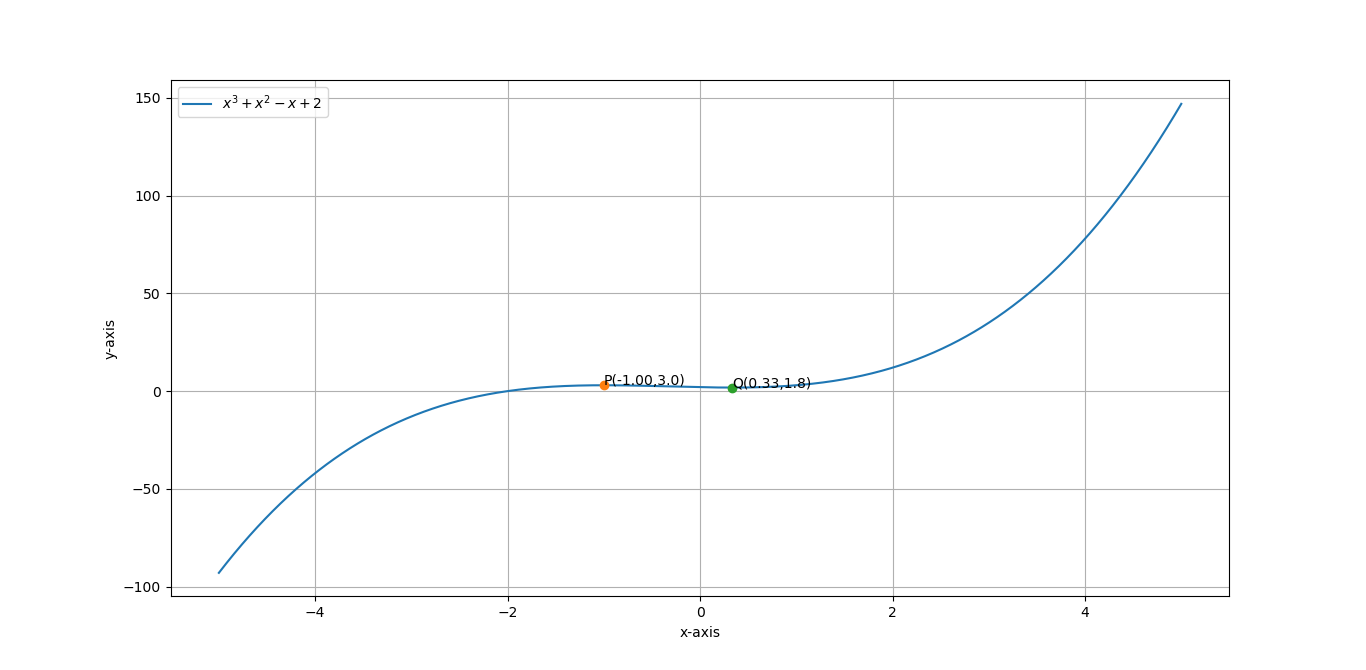
\includegraphics[scale=0.35]{opt.png}  

\textbf{Download code}

\begin{table}[h]
\large
\centering
\framebox{
\url{https://github.com/Siva Krishna/blob/main/conics/code/conic.py}}
\bibliographystyle{ieeetr}
\end{table} 
\end{multicols}
\end{document}
